\section{Theorie}
\label{sec:Theorie}

\subsection{Zeeman-Effekt}
\begin{figure}
  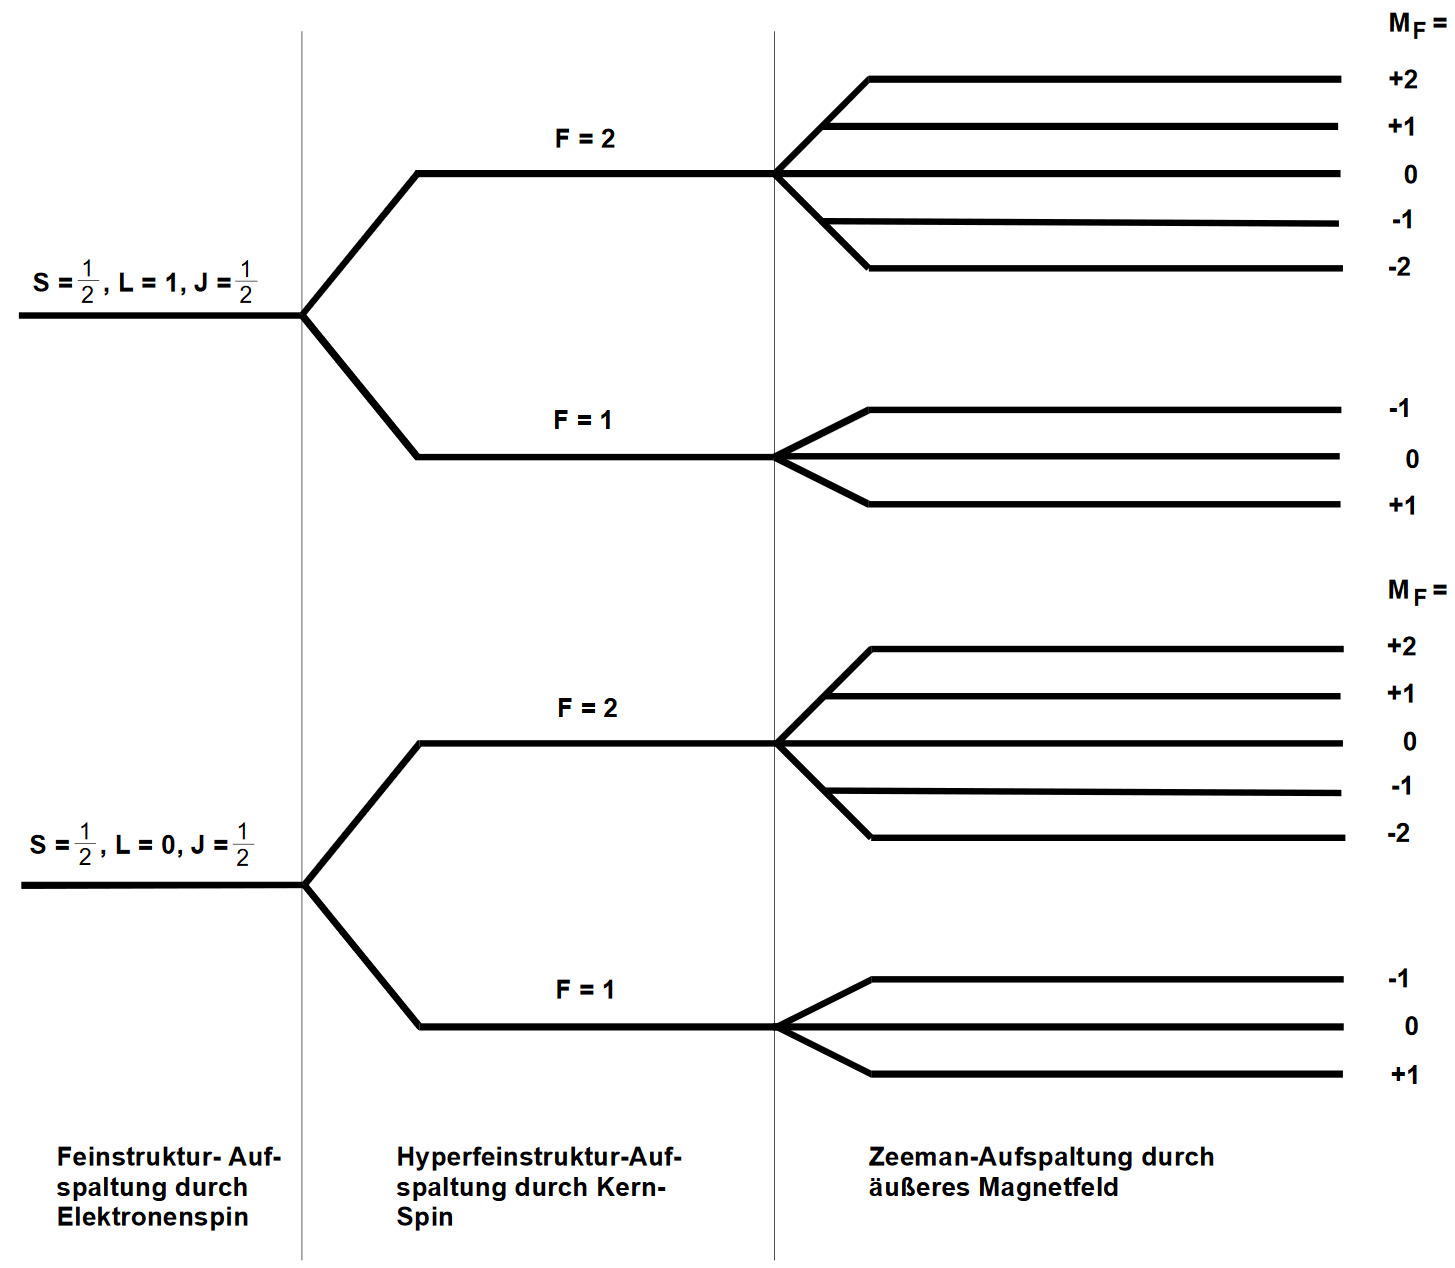
\includegraphics{./Niveaus.PNG}
  \caption{\cite{Anleitung}}
  \label{fig:Zeemann}
\end{figure}
Der sog. Zeeman-Effekt beschreibt die Aufspaltung der Energieniveaus von Atomen unter Einfluss eines äußeren Magnetfeldes.
Sein Ursprung liegt im magnetischen Moment $\mu_F$ der Atome, welches durch den Gesamtdrehimpuls
\begin{equation}
  \vec{\text{F}}=\vec{\text{L}}+\vec{\text{S}}+\vec{\mathbf{I}}
  \label{eqn:F}
\end{equation}
hervorgerufen wird. $\vec{\text{L}}$ bezeichnet hierbei den Bahndrehimpuls der Hüllenelektronen, $\vec{\text{S}}$ ihren Spin und $\vec{\mathbf{I}}$ den Kernspin. Diese Kopllung ist in Abb. \ref{fig:F} graphisch dargestellt.
Über die Quantenzahl $|I-J|<\text{F}<I+J$ lässt sich das Magnetische Moment nun durch

\begin{equation}
  \mu_F = \mu_B \text{g}_\text{F} \sqrt{F(F+1)}
  \label{eqn:mu_F}
\end{equation}
berechnen, wobei $\mu_B$ das Bohrsche Magneton und $\text{g}_\text{F}$  den sogenannten Landéfaktor bezeichnet.
\begin{figure}
  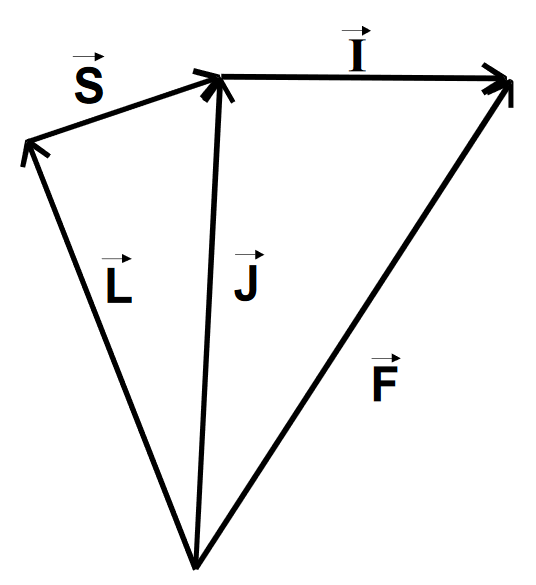
\includegraphics{./Kopplung.PNG}
  \caption{\cite{Anleitung}}
  \label{fig:F}
\end{figure}
Dieses Moment sorgt dafür, dass bei einem äußeren Magnetfeld $B$ die Energieniveaus der durch den Kernspin hervorgerufenen Hyperfeinstruktur in $2\text{F}-1$ durch eine weitere Quantenzahl $-\text{F}<\text{m}_\text{F}<\text{F}$ identifizierbare Zeeman-Niveaus aufgespalten werden. Für die Energiedifferenz zwischen benachbarten Zeeman-Niveaus gilt
\begin{equation}
  U_{Z}=\text{g}_\text{F}\mu_B B
  \label{eqn:U}
\end{equation}
Eine schematische Darstellung dieser Aufspaltung ist in Abb. \ref{fig:Zeemann} für $\mathbf{I}= \frac{2}{3}$ gegeben.
$\text{g}_\text{F}$ lässt sich mit einigen Vorüberlegungen aus den Drehimpulsquantenzahlen sowie des kernspinfreien Landé-Faktors $\text{g}_\text{J}$ durch
\begin{equation}
  \text{g}_\text{F} \approx  \text{g}_\text{J} \frac{\text{F}\left(\text{F}+1\right)+\text{J}\left(\text{J}+1\right)-\mathbf{I}\left(\mathbf{I}+1\right)}{2\text{F}\left(\text{F}+1\right)}
  \label{eqn:gf}
\end{equation}
berechnen.
Für $\text{g}_\text{J}$ gilt hierbei
\begin{equation}
  \text{g}_\text{J} = \frac{(1+\text{g}_\text{s})\text{J}\left(\text{J}+1\right)+(1-\text{g}_\text{s})\left(\text{S}\left(\text{S}+1\right)-\text{L}\left(\text{L}+1\right)\right)}{2\text{J}\left(\text{J}+1\right)}.
  \label{eqn:gj}
\end{equation}
$\text{g}_\text{s}\approx 2,0023$ bezeichnet den Landéfaktor des freien Elektrons.

\subsection{Optisches Pumpen}
Beim Vorgang des optisches Pumpens wird ausgenutzt, dass für durch Photonenabsorbtion hervorgerufene Zustandsänderungen gewisse Auswahlregeln gelten.
Diese betreffen die Polarisierung des einfallenden Lichtes, da linearpolarisiertes Licht $m=0$, zirkularpolarisiertes jedoch $m=\pm1$ in das Atom trägt. Durch geeignete Wahl der Photonenenergien können hierdurch nicht nur einzelne Feinstrukturniveaus, sondern auch einzelne Zeemann-Niveaus gesondert behandelt werden.
Strahlt man beispielsweise nur Licht der D1-Spektrallinie des Rubidium auf eine Rubidiumprobe, so sind in diesem ausschließlich Anregungsübergänge zwischen dem $^2{S}_{1/2}$- und dem $^2{P}_{1/2}$-Zustand möglich. Wählt man nun rechtszirkularpolarisiertes Licht, so muss für jede Anregung $\Delta_{m_{\text{F}}}=+1$ gelten. Dies bedeutet, dass Elektronen, welche sich im $^2{S}_{1/2}$-Zustand mit $\text{F}=m_{\text{F}}=2$ befinden nicht anregen lassen, da es keinen $^2{P}_{1/2}$-Zustand mit $m_{\text{F}}=3$ gibt. Alle übrigen $^2{S}_{1/2}$ Elektronen werden angeregt, emittieren ein Photon und kehren in einen \textit{beliebigen} $^2{S}_{1/2}$-Zustand zurück. Innerhalb der Zeemann-Niveaus eines Zustandes sind spontane Photonenemissionen sehr selten, weshalb sich das $\text{F}=m_{\text{F}}=2$ Niveau des $^2{S}_{1/2}$-Zustandes über die Zeit mit Elektronen füllt.
Sie verlassen diesen Zustand erst, wenn eine sogenannte \textit{induzierte Emission} auftritt, d.h. wenn bereits ein Photon der Energie $h\nu = U_{Z}$ auftritt. In diesem Fall ist es einem $m_{\text{F}}=2$-Elektron möglich, ein identisches Photon zu emittieren.
